\chapter{Finite Element Interface}
\label{ch-FEI}

\section{Introduction}

Many application codes use unstructured finite element meshes.
This section describes an interface for finite element problems,
called the {\tt FEI}, which is supported in \hypre{}.
\begin{figure}[htbp]
\centerline{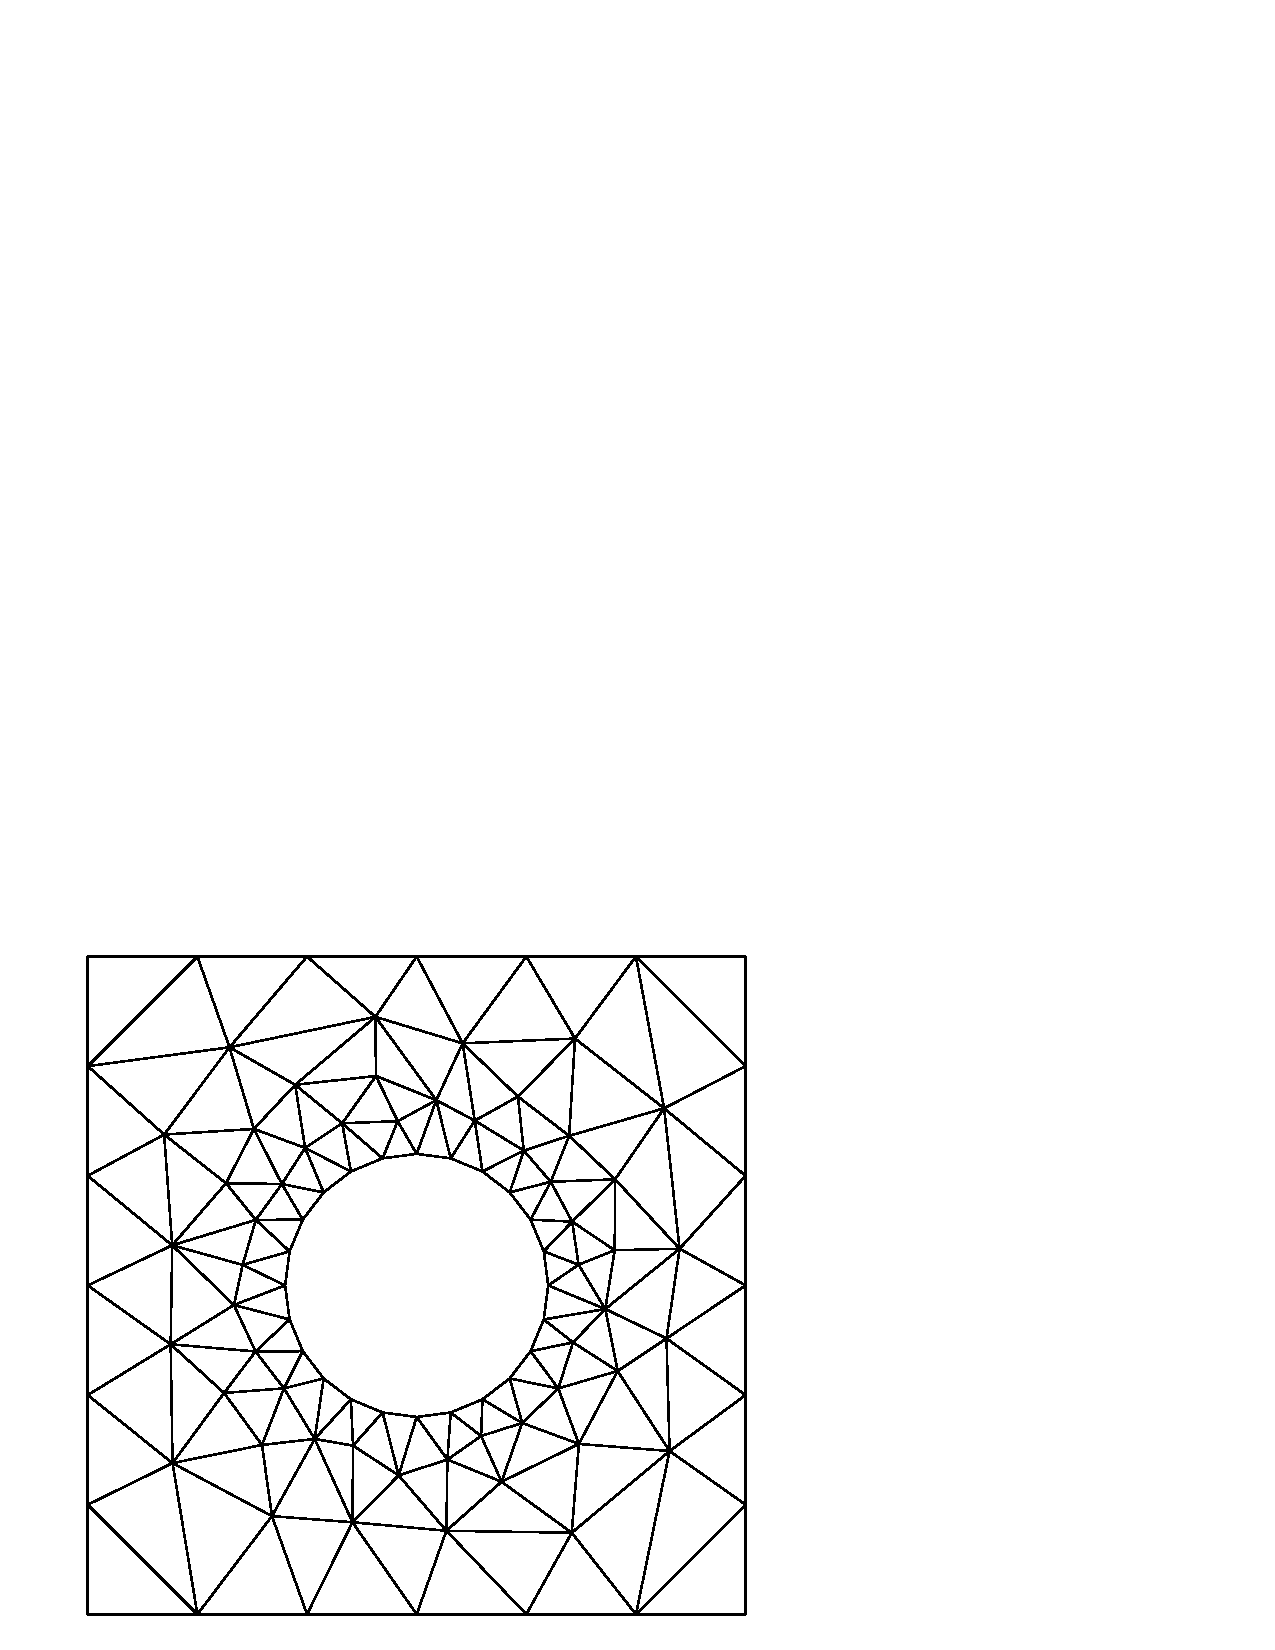
\includegraphics[width=.3\textwidth]{square-hole.pdf}}
\caption{Example of an unstructured mesh.}
\end{figure}

{\tt FEI} refers to a specific interface for black-box finite element
solvers, originally developed in Sandia National Lab, see \cite{FEI-ref}.
It differs from the rest of the conceptual interfaces in
\hypre{} in two important aspects: it is written in C++, and
it does not separate the construction of the linear system matrix
from the solution process.
A complete description of Sandia's {\tt FEI} implementation can be obtained
by contacting Alan Williams at Sandia (william@sandia.gov).
A simplified version of the {\tt FEI} has been implemented
at LLNL and is included in \hypre{}.
More details about this implementation can be found in the header
files of the \code{FEI_mv/fei-base} and \code{FEI_mv/fei-hypre} directories.

%% The purpose of the {\tt FEI} is to allow users to submit the global
%% matrices in the form of element connectivities, element stiffness matrices,
%% element loads, and boundary conditions.
%% The element information is processed by an implementation of the
%% {\tt FEI} (see \cite{FEI-ref}) which loads the global matrix and right
%% hand side vectors to the linear solver libraries via the
%% {\tt LinearSystemCore} interface.

%% In the next section, we 
%% describe the basic {\tt FEI} functions and a sample program to 
%% demonstrate how to use them. 


%% User applications access the \hypre{} linear solvers via a pipeline of
%% two interfaces - user to finite element interface (called {\tt FEI}),
%% and the finite element to linear solver interface (called 
%% {\tt LinearSystemCore}). The purpose of {\tt FEI} is to allow users 
%% to submit the global matrices in the form of element connectivities, 
%% element stiffness matrices, element loads, and boundary conditions. 
%% The element information is processed by an implementation of the 
%% {\tt FEI} (see \cite{FEI-ref}) which loads the global matrix and right
%% hand side vectors to the linear solver libraries via the 
%% {\tt LinearSystemCore} interface.
%% The {\tt LinearSystemCore} interface also facilitates interfacing 
%% multiple linear system solver packages (such as PetSC or Aztec)
%% with little change in the user code. Users interact with an FEI
%% solver primarily at the FEI level.

%% The specification of the {\tt FEI} and its implementation was first
%% developed at Sandia. A simplified implementation has been implemented
%% at LLNL in \hypre{}'s finite element module. While most of \hypre{}
%% is written in C, the {\tt FEI} and {\tt LinearSystemCore}
%% interfaces are written in C++. In the next section, we 
%% describe the basic {\tt FEI} functions and a sample program to 
%% demonstrate how to use them. 

%A brief description of \hypre{}'s 
%internal data structure and solver capabilities is presented in 
%Section 5.3.  Associated with \hypre{}'s finite element interface is 
%an FE-based gray-box multilevel preconditioning module called 
%{\tt MLI} which provides fast multilevel preconditioners.
%A description of the {\tt MLI} is given in Section 5.4.
%In Section 5.5, we describe the available options for using \hypre{}'s
%rich solver capabilities. 
%Users who prefer to create their own finite
%element packages but would like to use the \hypre{} solvers can link their
%packages to \hypre{} via the {\tt LinearSystemCore}. A description
%of this interface is given in Section \ref{LSI_overview}. Some installation 
%and usage issues are discussed in Section \ref{LSI_install}.

\section{A Brief Description of the Finite Element Interface}

Typically, finite element codes contain data structures storing element
connectivities, element stiffness matrices, element loads, boundary conditions,
nodal coordinates, etc.
One of the purposes of the {\tt FEI} is to assemble the global linear
system in parallel based on such local element data.
We illustrate this in the rest of the section and refer to example 10
(in the \code{examples} directory) for more implementation details.

In \hypre{}, one creates an instance of the {\tt FEI} as follows:
\begin{display}
\begin{verbatim}
LLNL_FEI_Impl *feiPtr = new LLNL_FEI_Impl(mpiComm);
\end{verbatim}
\end{display}
Here {\tt mpiComm} is an MPI communicator (e.g. {\tt MPI\_COMM\_WORLD}).
If Sandia's {\tt FEI} package is to be used, one needs to define
a \hypre{} solver object first:
\begin{display}
\begin{verbatim}
LinearSystemCore   *solver = HYPRE_base_create(mpiComm);
FEI_Implementation *feiPtr = FEI_Implementation(solver,mpiComm,rank);
\end{verbatim}
\end{display}
where {\tt rank} is the number of the master processor (used only
to identify which processor will produce the screen outputs).
The \code{LinearSystemCore} class is the part of the \code{FEI} which
interfaces with the linear solver library. It will be discussed later in
Sections \ref{LSI_solvers} and \ref{LSI_install}.

Local finite element information is passed to the {\tt FEI} using
several methods of the \code{feiPtr} object.
The first entity to be submitted is the {\it field} information. 
A {\it field} has an identifier called {\tt fieldID} and a rank or
{\tt fieldSize} (number of degree of freedom). For example, a discretization
of the Navier Stokes equations in 3D can consist of velocity vector having
$3$ degrees of freedom in every node (vertex) of the mesh and a scalar pressure
variable, which is constant over each element. If these are the only variables,
and if we assign {\tt fieldID}s $7$ and $8$ to them, respectively, then the
finite element field information can be set up by
\begin{display}
\begin{verbatim}
nFields   = 2;                 /* number of unknown fields */
fieldID   = new int[nFields];  /* field identifiers */
fieldSize = new int[nFields];  /* vector dimension of each field */

/* velocity (a 3D vector) */
fieldID[0]   = 7;
fieldSize[0] = 3;

/* pressure (a scalar function) */
fieldID[1]   = 8;
fieldSize[1] = 1;

feiPtr -> initFields(nFields, fieldSize, fieldID);
\end{verbatim}
\end{display}

Once the field information has been established, we are ready to initialize
an element block. An element block is characterized by the block identifier,
the number of elements, the number of nodes per element, the nodal fields 
and the element fields (fields that have been defined previously). Suppose 
we use $1000$ hexahedral elements in the element block $0$, the setup 
consists of
\begin{display}
\begin{verbatim}
elemBlkID  = 0;     /* identifier for a block of elements */
nElems     = 1000;  /* number of elements in the block */
elemNNodes = 8;     /* number of nodes per element */

/* nodal-based field for the velocity */
nodeNFields     = 1;
nodeFieldIDs    = new[nodeNFields];
nodeFieldIDs[0] = fieldID[0];

/* element-based field for the pressure */
elemNFields     = 1;
elemFieldIDs    = new[elemNFields];
elemFieldIDs[0] = fieldID[1];

feiPtr -> initElemBlock(elemBlkID, nElems, elemNNodes, nodeNFields,
                        nodeFieldIDs, elemNFields, elemFieldIDs, 0);
\end{verbatim}
\end{display}
The last argument above specifies how the dependent variables are arranged in
the element matrices. A value of $0$ indicates that each variable is to be
arranged in a separate block (as opposed to interleaving).

In a parallel environment, each processor has one or more element blocks.
Unless the element blocks are all disjoint, some of them
share a common set of nodes on the subdomain boundaries. To facilitate
setting up interprocessor communications, shared nodes between subdomains
on different processors are to be identified and sent to the {\tt FEI}.
Hence, each node in the whole domain is assigned a unique global
identifier. The shared node list on each processor contains a subset
of the global node list
corresponding to the local nodes that are shared with the other processors.
The syntax for setting up the shared nodes is
\begin{display}
\begin{verbatim}
feiPtr -> initSharedNodes(nShared, sharedIDs, sharedLengs, sharedProcs);
\end{verbatim}
\end{display}
This completes the initialization phase, and a completion signal is sent to
the {\tt FEI} via
\begin{display}
\begin{verbatim}
feiPtr -> initComplete();
\end{verbatim}
\end{display}

Next, we begin the {\it load} phase. The first entity for loading is the
nodal boundary conditions. Here we need to specify the number of boundary
equations and the boundary values given by {\tt alpha, beta}, and {\tt gamma}.  Depending on whether the boundary conditions are Dirichlet, Neumann, or mixed,
the three values should be passed into the {\tt FEI} accordingly. 
\begin{display}
\begin{verbatim}
feiPtr -> loadNodeBCs(nBCs, BCEqn, fieldID, alpha, beta, gamma);
\end{verbatim}
\end{display}
The element stiffness matrices are to be loaded in the next step. We need
to specify the element number $i$, the element block to which element $i$
belongs, the element connectivity information, the element load, and the
element matrix format. The element connectivity specifies a set of $8$ node
global IDs (for hexahedral elements), and the element load is the load or
force for each degree of freedom.  The element format specifies how the
equations are arranged (similar to the interleaving scheme mentioned above).
The calling sequence for loading element stiffness matrices is
\begin{display}
\begin{verbatim}
for (i = 0; i < nElems; i++)
   feiPtr -> sumInElem(elemBlkID, elemID, elemConn[i], elemStiff[i],
                       elemLoads[i], elemFormat);
\end{verbatim}
\end{display}
To complete the assembling of the global stiffness matrix and the
corresponding right hand side, a signal is sent to the {\tt FEI} via
\begin{display}
\begin{verbatim}
feiPtr -> loadComplete();
\end{verbatim}
\end{display}

%% \section{The Finite Element Interface Matrix and Vector Classes}

%% This section describes two additional classes (other than {\tt HYPRE\_FEMesh})
%% that users may need - {\tt HYPRE\_FEMatrix} and {\tt HYPRE\_FEVector}. 
%% These classes are useful if the global finite element stiffness matrix is
%% to be solved using solvers other than those available via the finite element
%% interface. The key task is to extract
%% the matrix and vector internal to the {\tt FEI}. The matrix can be extracted
%% by first instantiating an {\tt HYPRE\_FEMatrix} object
%% \begin{tabbing}
%% \hspace{0.5in} \= {\tt HYPRE\_FEMatrixCreate(mpiComm, hypreMesh, \&feMatrix);}
%% \end{tabbing}
%% where {\tt hypreMesh} is the object created before, and {\tt feMatrix} is 
%% the pointer to the new object.
%% The \hypre{} matrix in {\tt ParCSR} format can then be extracted by
%% \begin{tabbing}
%% \hspace{0.5in} \= {\tt HYPRE\_FEMatrixGetObject(feMatrix, (void **) \&parcsrMatrix);}
%% \end{tabbing}
%% Similarly, the right hand side vector can be extracted by
%% \begin{tabbing}
%% \hspace{0.5in} \= {\tt HYPRE\_FEVectorCreate(mpiComm, hypreMesh, \&feVector);}
%% \end{tabbing}
%% and
%% \begin{tabbing}
%% \hspace{0.5in} \= {\tt HYPRE\_FEVectorGetRHS(feMatrix, (void**) \&parVectorRHS);}
%% \end{tabbing}
%% When the solution of the linear system is obtained, it can be given
%% to the {\tt FEI} by
%% \begin{tabbing}
%% \hspace{0.5in} \= {\tt HYPRE\_FEVectorSetSol(feMatrix, (void*) parVectorSol);}
%% \end{tabbing}
%% Finally, the objects are destroyed by the corresponding destroy functions.

%\section{The LinearSystemCore Interface}
%\label{LSI_overview}

%As described before, users who prefer to create their own finite element
%interface package can also take advantage of the rich solver capabilities
%in \hypre{}. In this section we show how to access {\tt HYPRE\_LinSysCore}'s
%internal solver directly.  
%The matrix class in \hypre{} accessible via the {\tt LinearSystemCore} interface
%is the parallel compressed sparse row ({\tt ParCSR}) matrix.  The
%requirements about how the global matrix is partitioned among the
%processors are that each processor holds a contiguous block of rows and columns
%and the equation numbers in processors of lower rank are lower than those
%in processors of higher rank.  The {\tt FEI} is responsible for ensuring
%that these two requirements are followed. The matrix can be loaded in
%parallel - a row or a block of rows at a time.  The solution and right
%hand side vectors are constructed accordingly. The matrix rows corresponding
%to the shared nodes can be assigned to either processor, and is determined
%by the {\tt FEI} itself. Once the incoming matrix and vector data have
%been captured in the \hypre{} {\tt ParCSR} format, a whole of matrix and
%vector operators are available for use in the \hypre{} solvers.
%
%The following program segment describes the function calls to set up
%the internal matrix and solve the linear system.
%Users need first to 
%construct an array (say, {\tt eqnOffsets} describing the matrix row
%partitioning across all processors (so {\tt eqnOffsets[p]} and
%{\tt eqnOffset[p+1]} have the starting and ending row indices for processor
%p). Furthermore, suppose the local submatrix has been constructed as a
%compressed sparse row (CSR) matrix in the {\tt ia, ja, val} arrays. 
%
%\begin{tabbing}
%\hspace{0.5in} \= {\tt Program Segment} \\[1mm]
%\> {\tt startRow = eqnOffsets[mypid];} \\
%\> {\tt endRow = eqnOffsets[mypid+1] - 1;} \\
%\> {\tt nrows = endRow - startRow + 1} \\
%\> {\tt for ( i = startRow; i $<=$ endRow; i++ ) $\{$ } \\
%\> \hspace{0.3in} \= {\tt ncnt = ia[i+1] - ia[i];} \\
%\> \> {\tt rowLengths[i-startRow] = ncnt;} \\
%\> \> {\tt colIndices[i-startRow] = new int[ncnt];} \\
%\> \> {\tt k = 0;} \\
%\> \> {\tt for (j = ia[i]; j < ia[i+1]; j++) colIndices[i-startRow][k++] = ja[j];}\\
%\> \} \\
%\> {\tt HYPRE\_LinSysCore\_create(\&lsc, MPI\_COMM\_WORLD);} \\
%\> {\tt HYPRE\_setGlobalOffsets(lsc, nrows, NULL, eqnOffsets, NULL);} \\
%\> {\tt HYPRE\_setMatrixStructure(lsc, colIndices, rowLengths, NULL, NULL, NULL);} \\
%\> {\tt for ( i = startRow; i <= endRow; i++ ) $\{$ } \\
%\> \> {\tt ncnt = ia[i+1] - ia[i];} \\
%\> \> {\tt HYPRE\_sumIntoSystemMatrix(lsc, i, ncnt, \&val[ia[i]], \&ja[ia[i]]);}\\
%\> \> {\tt HYPRE\_sumIntoRHSVector(1, \&rhs[i], \&i);} \\
%\> \} \\
%\> {\tt HYPRE\_matrixLoadComplete();}\\
%\> {\tt strcpy(paramString, "solver gmres");} \\
%\> {\tt HYPRE\_parameters(1, \&paramString);} \\
%\> {\tt strcpy(paramString, "preconditioner boomeramg");} \\
%\> {\tt HYPRE\_parameters(1, \&paramString);} \\
%\> {\tt HYPRE\_launchSolver(\&status, \&iterations);}
%\end{tabbing}

%A list of available functions is given in the reference manual.
%
%\begin{tabbing}
%{\tt HYPRE\_LinSysCore\_create(LinSysCore **lsc, MPI\_Comm comm)} \\[1mm]
%{\tt HYPRE\_LinSysCore\_destroy(LinSysCore **lsc)} \\[1mm]
%{\tt HYPRE\_parameters(LinSysCore *lsc, int nParams, char **params)} \\[1mm]
%{\tt HYPRE\_setGlobalOffsets(LinSysCore* lsc, int leng, int* nodeOffsets,} \\
%\hspace{1.0in} {\tt int* eqnOffsets, int* blkEqnOffsets)} \\[1mm]
%{\tt HYPRE\_setMatrixStructure(LinSysCore *lsc, int** ptColIndices,} \\
%\hspace{1.0in} {\tt int* ptRowLengths, int** blkColIndices, int* blkRowLengths, int* ptRowsPerBlkRow)} \\[1mm]
%{\tt HYPRE\_resetMatrixAndVector(LinSysCore *lsc, double val)} \\[1mm]
%{\tt HYPRE\_resetMatrix(LinSysCore *lsc, double val)} \\[1mm]
%{\tt HYPRE\_resetRHSVector(LinSysCore *lsc, double val)} \\[1mm]
%{\tt HYPRE\_sumIntoSystemMatrix(LinSysCore *lsc, int numPtRows, const int* ptRows,}\\
%\hspace{1.0in} {\tt int numPtCols, const int* ptCols, int numBlkRows, const int* blkRows,} \\
%\hspace{1.0in} {\tt int numBlkCols, const int* blkCols, const double* const* values)} \\[1mm]
%{\tt HYPRE\_sumIntoRHSVector(LinSysCore *lsc, int num, const double* values, const int* indices)} \\[1mm]
%{\tt HYPRE\_matrixLoadComplete(LinSysCore *lsc)} \\[1mm]
%{\tt HYPRE\_enforceEssentialBC(LinSysCore *lsc, int* globalEqn, double* alpha,
%                             double* gamma, int leng)} \\[1mm]
%
%{\tt HYPRE\_enforceRemoteEssBCs(LinSysCore *lsc,int numEqns,int* globalEqns, int** colIndices,} \\
%\hspace{1.0in} {\tt int* colIndLen, double** coefs)} \\[1mm]

%{\tt HYPRE\_enforceOtherBC(LinSysCore *lsc, int* globalEqn, double* alpha, double *beta} \\
%\hspace{1.0in} {\tt double* gamma, int leng)} \\[1mm]

%{\tt HYPRE\_putInitialGuess(LinSysCore *lsc, const int* eqnNumbers,
%                          const double* values, int leng)} \\[1mm]
%{\tt HYPRE\_getSolution(LinSysCore *lsc, double *answers, int leng)} \\[1mm]

%{\tt HYPRE\_getSolnEntry(LinSysCore *lsc, int eqnNumber, double *answer)} \\[1mm]

%{\tt HYPRE\_formResidual(LinSysCore *lsc, double *values, int leng)} \\[1mm]

%{\tt HYPRE\_launchSolver(LinSysCore *lsc, int *solveStatus, int *iter)} \\[1mm]
%\end{tabbing}

%\section{HYPRE LinearSystemCore Installation}
%
%The ultimate objective is for application users to have immediate access
%to the latest FEI/\hypre{} library files on different computing platforms
%via public {\tt lib} directories.  While this feature is forthcoming, careful 
%version control is needed for users to keep track of capabilities and bug fixes 
%for different installations.  Users who would like to set up the FEI/\hypre{}
%on their own should do the following :
%
%\begin{enumerate}
%
%\item obtain the \hypre{} and the Sandia FEI source codes (alternatively, use
%      the {\tt FEI} implementation in \hypre{}),
%\item compile Sandia's {\tt FEI} (fei-2.5.0) to create the
%      {\tt libfei\_base.a} file.
%\item compile \hypre{} 
%\begin{enumerate}
%\item download \hypre{} from the web, ungzip and untar it
%\item go into the {\tt linear\_solvers} directory
%\item do a 'configure' with the {\tt --with-fei-inc-dir} option set to
%      the {\tt FEI} include directory plus other compile options
%\item compile with {\tt make install} to create the
%      {\tt libHYPRE\_LSI*} file in the {\tt linear\_solvers/hypre/lib}
%      directory.
%\end{enumerate}
%\item call the {\tt FEI} functions in your application code (example given
%      previously)
%\begin{enumerate}
%\item include {\tt cfei\-hypre.h} in your file 
%\item include {\tt FEI\_Implementation.h} in your file 
%\item make sure your application has an {\tt include} and an {\tt lib} path 
%      to the {\tt include} and {\tt lib} directories created above. 
%\end{enumerate}
%
%\end{enumerate}
%
%%\subsection{Linking with the library files}
%
%To link the {\tt FEI} and \hypre{} into the executable, the following has to be
%attached to the linking command :
%
%\begin{tabbing}
%\hspace{0.5in} \= {\tt -L\$$\{$LIBPATHS$\}$ -lfei\_base -lHYPRE\_LSI} 
%\end{tabbing}
%along with all the other libraries (Note : the order in which the libraries are
%listed may be important), where {\tt LIBPATHS} are where 
%the \hypre{} and {\tt FEI} libraray files can be found.  
%
%Since some of these library files make calls to LAPACK and BLAS functions, 
%the corresponding libraries need to be linked along with (placed after) these 
%library files.  
%%For example, on the DEC cluster, it suffices to link
%%with the {\tt dxml} library, (So {\tt -ldxml} is placed after the above link
%%sequence, with {\tt -lm} placed after {\tt -ldxml}.) while the {\it essl}
%%library can be used on the blue machine. If {\tt SuperLU} is also needed,
%%{\tt -lHYPRE\_superlu} should be placed immediately after {\tt HYPRE\_LSI}.
%
%%\subsection{Some more caveats for application developers}
%
%Building an application executable often requires linking with many different
%software packages, and many software packages use some LAPACK and/or BLAS
%functions.  In order to alleviate the problem of multiply defined functions
%at link time, it is recommended that all software libraries are stripped of
%all LAPACK and BLAS function definitions.  These LAPACK and BLAS functions 
%should then be resolved at link time by linking with the system LAPACK and
%BLAS libraries (e.g. dxml on DEC cluster).  Both \hypre{} and SuperLU were
%built with this in mind.  However, some other software library files needed
%may have the BLAS functions defined in them.  To avoid the problem of
%multiply defined functions, it is recommended that the offending library
%files be stripped of the BLAS functions.
%
%%\subsection{Comments about the FEI/\hypre{} Interface and Contacts}
%
%%Comments about \hypre{}'s finite element interface can be directed
%%to Charles Tong (925-422-3411, chtong@llnl.gov).
%
